\chapter{The Milky Way as a Galaxy}\label{chap:milkyway}
\section{Components}\label{sec:components}
\begin{figure}[t]
    \centering
    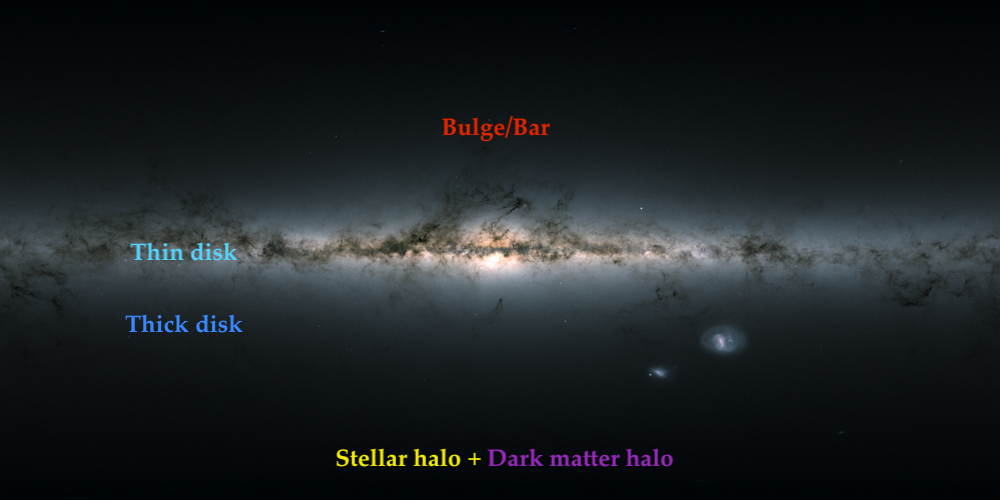
\includegraphics[width=1\textwidth]{images/gaiasky.png}
    \caption{All-sky view of the Milky Way Galaxy from Gaia based on measurements of nearly 1.7 billion stars. We mark the location of different components of the Galaxy with different colors. Image adapted from \textit{Gaia} Data processing and Analasys Consortium (DPAC) (CC BY-SA 3.0 IGO).} % Fig. 1.1
    \label{fig:gaiasky}
\end{figure}
All throughout history mankind has sought to understand the night sky and its many features such as stars, clumps, planets or `wanderers'. But no feature is as large and noticeable as the great spray of stars that make up the Milky Way Galaxy, named so for the milk from Hera's breast in Greek mythology \citep{leeming:98}. The suggestion that this milky band of stars was a rotating body, of which we the observers are inside, came not until \cite{wright:1750}. Since then our understanding of our home Galaxy has increased tremendously and we can present stunningly detailed views of it like the map shown in Fig. \ref{fig:gaiasky}. This map is made possible thanks to measurements from Gaia's second data release (\citealt{dr2},  herafter DR2). As the figure shows the Milky Way is composed of several different components with stars differing in spatial distribution, kinematics, chemistry, and age. Since the three papers together touch upon almost every component mentioned in Fig. \ref{fig:gaiasky} we will briefly provide a description of each one.

\subsection{Thin disk}\label{subsec:components-thindisk}
The thin disk is what visually makes up the Milky Way and since it is where the Sun is located it is the the most well-studied of the stellar components. The thin disk is also the site of ongoing star formation which recent estimates place as high as $\approx 3.3\ \mathrm{M_\odot yr}^{-1}$ \citep{zari:22}. As the name suggests it is relatively thin with a scale length of $R_\mathrm{t} \approx 2.6$ kpc, scale height of $z_\mathrm{t} \approx 300$ pc, and with a mass $M_\mathrm{t} \approx 3.5\times 10^10$ M$_\odot$ \citep{bland-hawthorn:16}. The thin disk stars are generally younger and has an abundance of $\alpha$-elements similar to the sun. We measure the abundances as:
\begin{equation}
    [\alpha/\mathrm{Fe}] = \log_{10}\left(\frac{N_\alpha}{N_\mathrm{Fe}}\right)_\mathrm{star} - \log_{10}\left(\frac{N_\alpha}{N_\mathrm{Fe}}\right)_\odot,
\end{equation}
where $N$ is the number of atoms per unit of volume.

\subsection{Thick disk}\label{subsec:components-thickdisk}
The second disk of the Galaxy fulfills its name with a scale height of $z_\mathrm{T}\approx 900$ pc, scale length $R_\mathrm{T} \approx 2$ kpc, and mass $M_\mathrm{T} \approx 6$ M$_\odot$ \citep{bland-hawthorn:16}. It's stars are older \citep{martig:16} and kinematically hotter, since age and velocity dispersion are correlated (\citealt{martig:14,aumer:16}). In metallicity space, thick disc stars occupy regions of higher [$\alpha$/Fe] and have been tentatively linked to the high-$\alpha$ sequence \citep{katz:21}. How the thick and thin discs formed is still a debated topic, particularly so the former as explained in \cite{helmi:20} who also shows that the formation may be related to the evolution of the stellar halo through mergers with nearby galaxies. 

\subsection{Stellar halo}\label{subsec:components-stellarhalo}
The most extended component is the stellar halo which contains $1.3^{+0.3}_{-0.2} \times 10^9$ M$_\odot$ within $2 < r < 70$ kpc \citep{mackereth:20} and is host to the oldest and most metal-poor stars in the Galaxy \citep{dacosta:19, horta:22}. The orbits of halo stars is more spherical than the disks and so can be told apart locally by their kinematics. Relative to the discs, the halo stars will appear to move with a speed of 200 km s$^{-1}$. The most commonly held formation pathway for the Milky Way is through hierarchical growth through several minor and major mergers, a model called $\Lambda$CDM \citep{springel:05}. This view matches well with current understanding of the stellar halo as having an \textit{in situ} component of stars as well as an accreted component which becomes extremely dominant at larger distances from the disk \citep{naidu:20}. It has also been shown that this accreted component has a plethora of substructures in it attributed to various accreted stellar populations (e. g. \citealt{koppelman:19, feuillet:21, dodd:22}). We will touch more upon this in sections \ref{sec:p3-gaiaview} and \ref{sec:p3-structures}.

\subsection{Dark matter halo}\label{subsec:components-darkhalo}
There is another halo which is not visible to our telescopes. If we only look to the stellar matter of a galaxy like the Milky Way, the rotational velocity of stars is expected to decrease with distance in a similar fashion to Keplerian rotation, in which $v_\mathrm{rot}^2 \propto M/R$. This is not what we observe however, and instead the rotation curve flattens out which is attributed to the existence of a dark matter halo. Current results place the mass of the dark matter halo at $M_\mathrm{dh} \approx 1.3 \times 10^12$ M$_\odot$ \cite{posti:19} and its shape is still a topic of much debate as explained in \cite{mcmillan:17}. While the debate goes on, it is very common in simulations to assume a spherically symmetric halo (e. g. \citealt{andersson:20}).

\subsection{The bulge}\label{subsec:components-bulge}
In the central regions of the Galaxy lies the bulge, heavily obscured by dust as is clearly visible in Fig. \ref{fig:gaiasky}. The nature of the bulge \textit{as a bulge} is uncertain. The idea of a spherical, so-called \textit{classical bulge} built up through early mergers makes sense given the old ages of bulge stars \citep{clarkson:08}. Following star counts in the bulge, it has been established that the bulk of the bar participates in a \textit{box/peanut}-shaped structure, related to the three-dimensional Galactic \textbf with cylindrical rotation (\citealt{wegg:13, ness:13b}). It us unclear if the Milky Way even has a classical bar. \cite{shen:10} uses the kinematics to constrain its contribution to be less than 8\% of the disk mass and it has been shown that the bulge has several different metallicity populations \citep{ness:13a}. There is evidence to suggest that parts of the bulge is formed from the Galactic disk \citep{dimatteo:19} through interactions that slowly rearrange energy, angular momentum, and mass, otherwise known as \textit{secular evolution} \citep{kormendy:13}.

\section{The bar \& spiral arms}\label{sec:barspirals}
\begin{figure}[t]
    \centering
    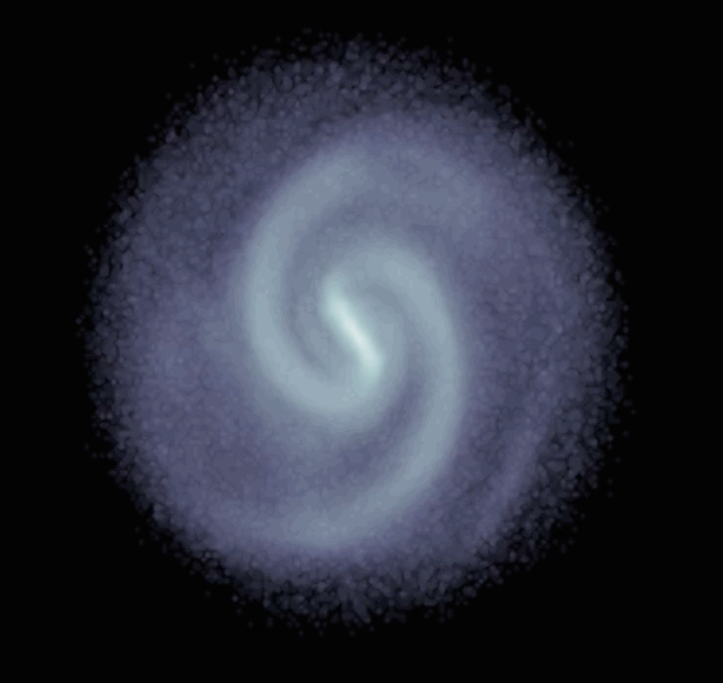
\includegraphics[width=.65\textwidth]{images/simgal.png}
    \caption{An example of a simulated Milky-Way like disc Galaxy with pronounced spiral arms and a central bar.} % Fig. 1.2
    \label{fig:simgal}
\end{figure}
Beyond the components mentioned in the previous sections, there are the non-axisymmetric features. In other galaxies they are clearly visible but since we reside inside our Galaxy we struggle to see them as clearly. As an example we show a simulated galaxy in Fig. \ref{fig:simgal} which has a bar and two spiral arms that can be seen very clearly and represents a typical disc galaxy. Since non-axisymmetric features play an important role in secular evolution we will take a closer look at these features in the Milky Way.

The boxy/peanut shaped bulge mention in section \ref{subsec:components-bulge} is an inner, vertical extension of the Galactic bar \citep{bland-hawthorn:16}. The bulge region reaches to about ${\sim}2$ kpc \citep{wegg:13} while the bar may reach as far as 5 kpc \citep{wegg:15}. For this reason it is sometimes referred to as the `long' bar. Current estimates for the bar puts it at ${\sim}1.6\pm 0.3 \times 10^10$ M$_\odot$ \citep{kipper:20} and using Gaia's third data release (\citealt{dr3}, hereafter DR3) the bar angle with respect to the Sun-Galactic Centre (GC) is estimated to be $-19.2^\circ \pm 1.5^\circ$ \citep{dr3:asymmetries}. The bar is not static however and is rotating with a specific angular velocity, called pattern speed. The pattern speed of the bar is subject to much debate with many attempts at determining it. In \cite{bland-hawthorn:16} they review many of the estimates and conclude with an estimated pattern speed of $\Omega_\mathrm{b} \simeq 43 \pm 9$ km s$^{-1}$ kpc$^{-1}$. More recent estimates place the pattern speed of the bar at $\Omega_\mathrm{b} = 33.29 \pm 1.81$ km s$^{-1}$ kpc$^{-1}$ \citep{clarke:22}, in agreement with the previous value. These scales of pattern speeds has been called a `slow' bar scenario.

The other major non-axisymmetric feature of the Milky Way are the spiral arms. They likely travel around the whole disk and as such, we do not have a full picture of them to date and instead must look to whatever parts of them are visible to us from our position as observers in their plane. Current belief within the community is that the Milky Way has four approximately symmetric spiral arms \citep{vallee:17} rather than just two. The names for these four arms as in literature are \textit{Perseus}, \textit{Sagittarius-Carina}, \textit{Scutum-Centaurus}, and \textit{Norma-Outer}. The sun is believed to lie inside of \textit{Perseus}, and just outside \textit{Sagittarius-Carina} in an inter-arm region. In addition to these arms, very close to the Sun lies the \textit{local arm}, initially believed to be a spur of the \textit{Perseus arm}. It has since been understood to be fifth feature with comparable qualities to the other major arms. In spiral galaxies the highest densities of gas and stars lie along the arms which is the site for most star-formation in the disk. 

\section{Radial migration}\label{sec:migration}
\begin{figure}[t]
    \centering
    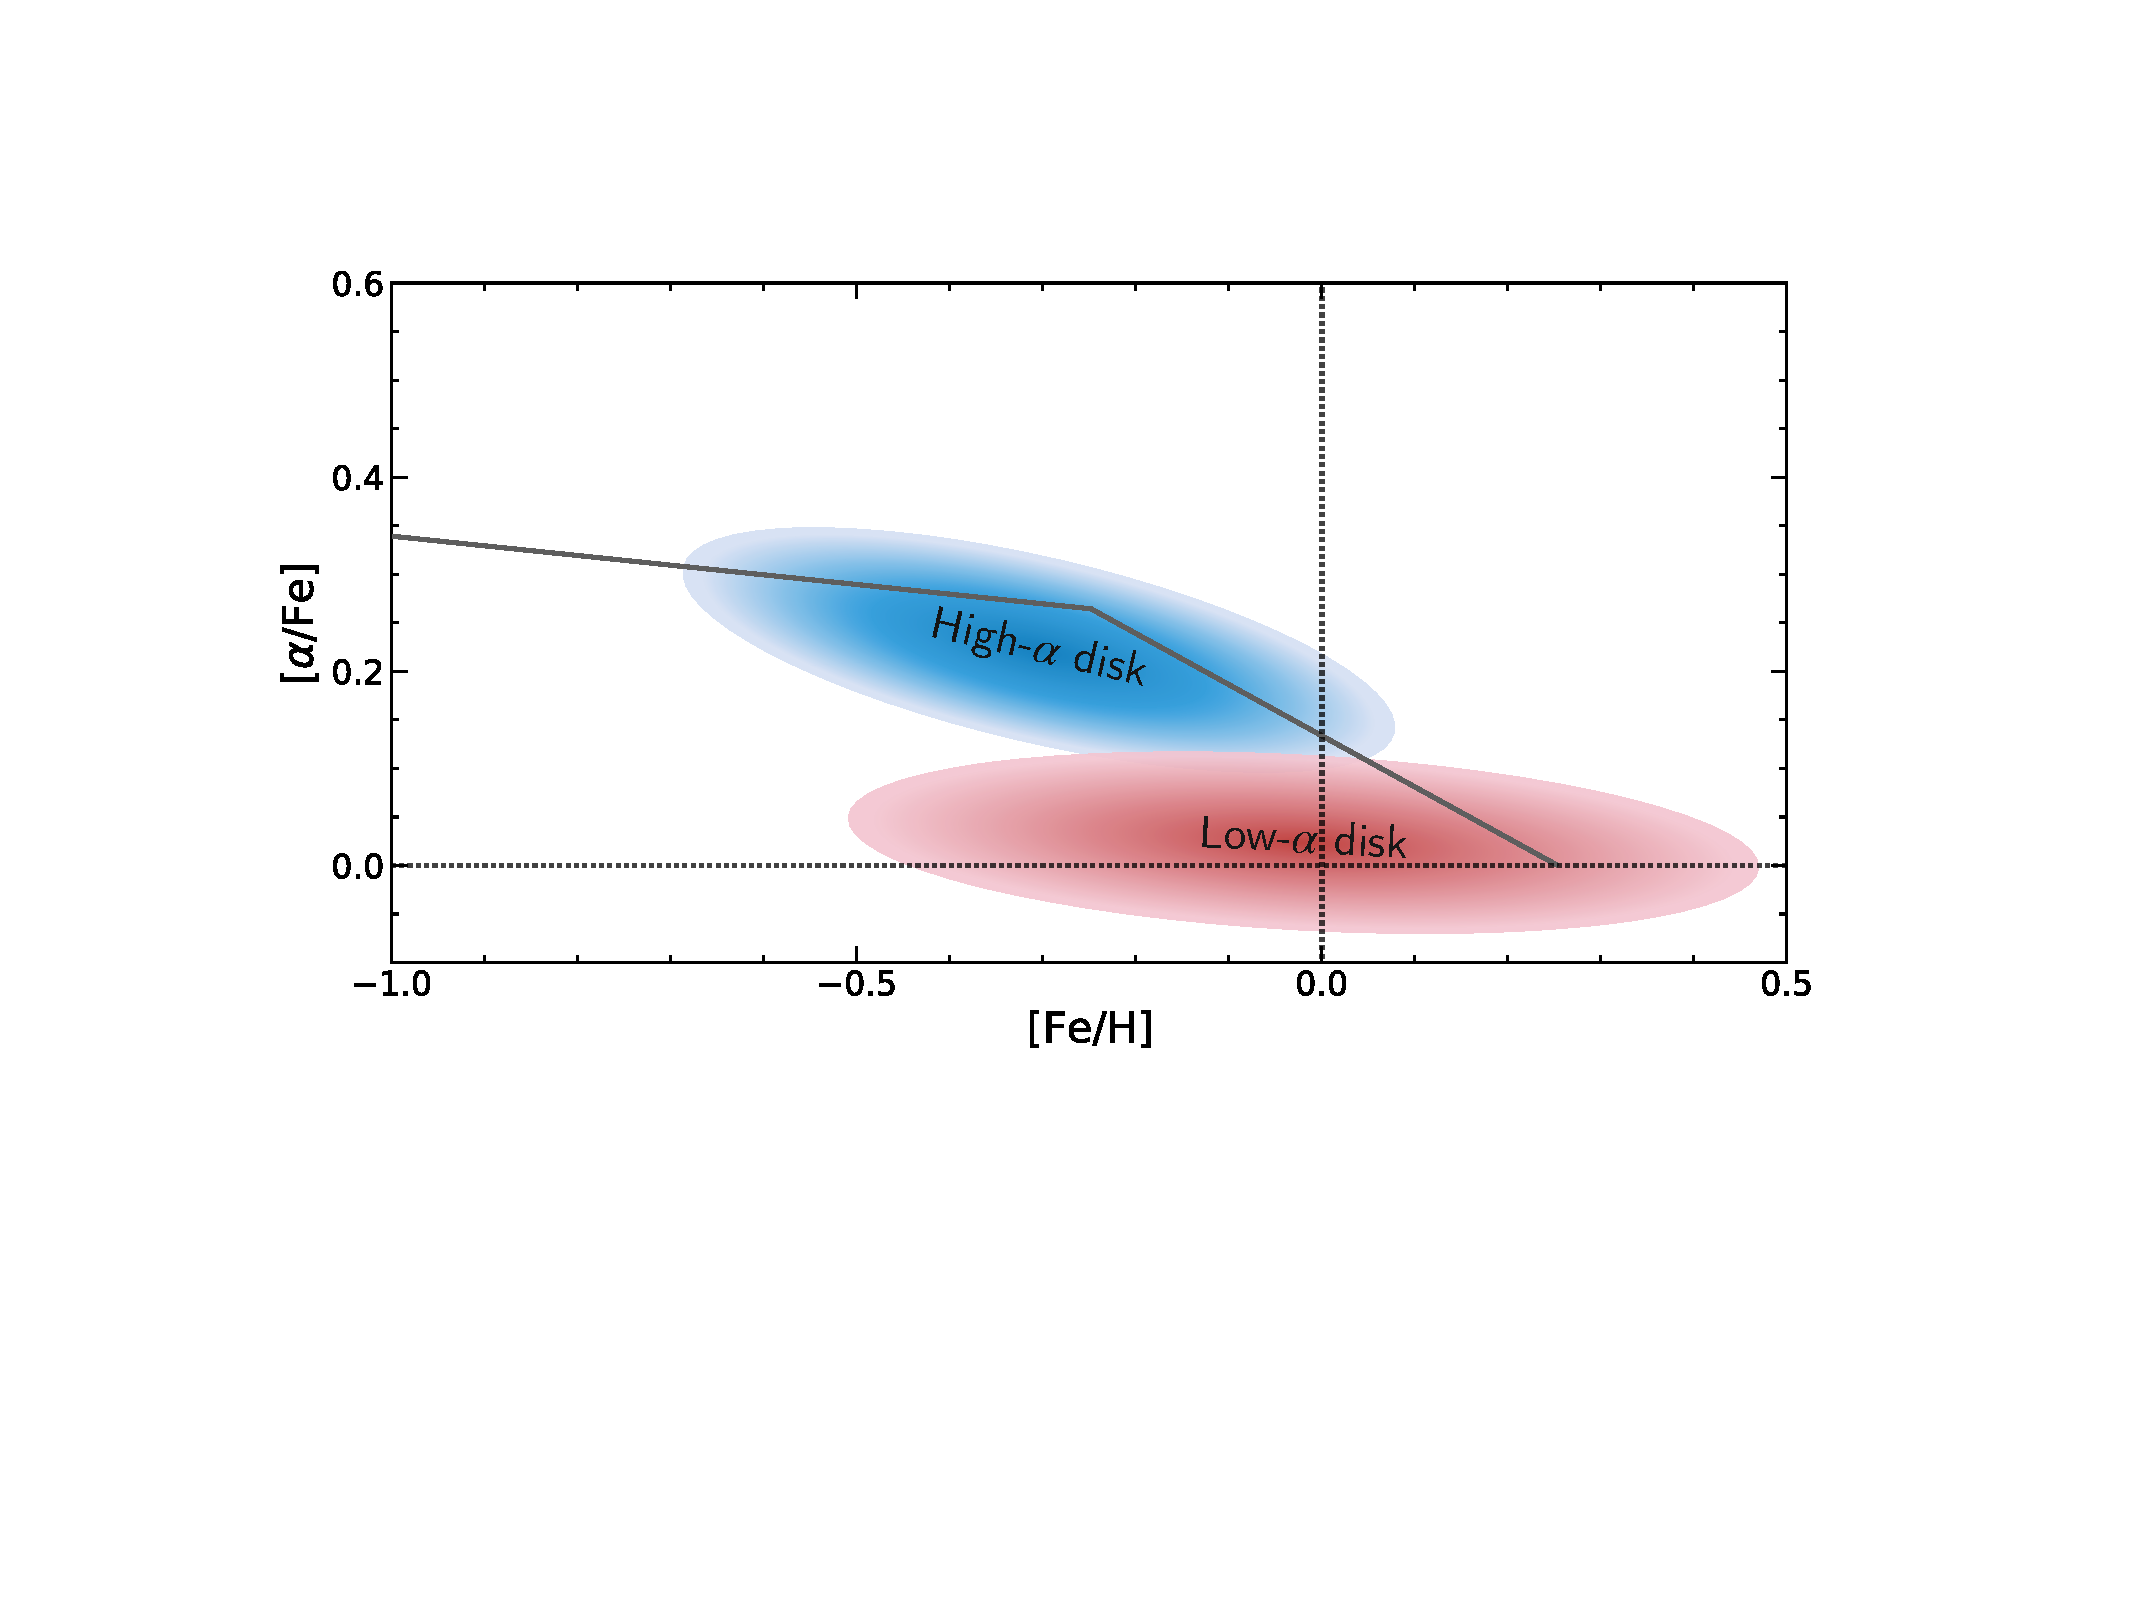
\includegraphics[width=.9\textwidth]{images/alphaoverfe.pdf}
    \caption{An illustration of the distribution of abundance of $\alpha$-elements vs the abundance of iron. The dotted line shows the location of the Sun and the gray solid line the expected evolution of an isolated region of the ISM.} % Fig. 1.3
    \label{fig:alphaoverfe}
\end{figure}
Since the spiral arms and the Galactic bar are such very prominent features of our Galaxy and in other similar spiral galaxies, it is no surprise that they have a profound impact upon the disc in which they are found and the stars that live therein. One such effect which occurs because of the dynamical interplay between disk and the non-axisymmetric features is \textit{radial migration}, which is the displacement of a star in the radial direction of its galactic plane. We will soon explain the mechanics of the major processes which cause radial migration but first the importance of radial migration as an ingredient of galaxy evolution, and the evidence to support it, should be discussed.

Let us consider the chemical evolution of the Galactic disc. The abundance of $\alpha$-elements and Fe over time in an isolated region of the interstellar matter (ISM) are affected by the life and death of its stars through what is called stellar nucleosynthesis (for a review see \citealt{edvardsson:1993}). In short, stars create elements and enhances the abundances of the next generation. Initially core-collapse supernovae produce similar amount of $\alpha$ and Fe, but [Fe/H] increases. Eventually type Ia supernovae begin, which produces Fe but no $\alpha$-elements and thus for the region [$\alpha$/Fe] starts to drop. This behaviour produces a trend like the gray line seen in Fig. \ref{fig:alphaoverfe}. If we are in a very isolated region, we would expect to see that the stars follow this narrow trend. Neighbouring regions radially inside and outside of the region would however have higher and lower [Fe/H] ranges as it has been shown that [Fe/H] increases radially inwards in the Galaxy \citep{hayden:15}. In observations of the Solar neighbourhood (e. g., \citealt{edvardsson:1993, hayden:15, bensby:14},) we see a range of different Fe abundances at each [$\alpha$/Fe], similar to the illustration shown in Fig. \ref{fig:alphaoverfe}. Similarly, the age-metallicity relationship (AMR) can be expected to follow a narrow line for this region, but shows a wide scatter. This can be quite easily explained if the different regions of the disc are not isolated from each other, but rather there is radial mixing between them. Beyond this rather straight-forward example of radial migration, several other observed features of the Milky Way disc has been suggested to be caused by it as well such as the observed bimodality in plots like Fig. \ref{fig:alphaoverfe} \citep{schonrich:09, toyouchi:2016} and the flaring of the outer disk in mono-age populations \citep{minchev:12}. It is clear that some form of radial migration is occurs in the Milky Way and we are today even able to estimate the radial displacement of individual stars as in \cite{frankel:18} which finds that the Sun as well has likely migrated from a birth radius of {$\sim$}5.2 kpc. Therefore it is important to understand the processes by which migration occurs.

\subsection{Radial heating}
\begin{figure}[t]
    \centering
    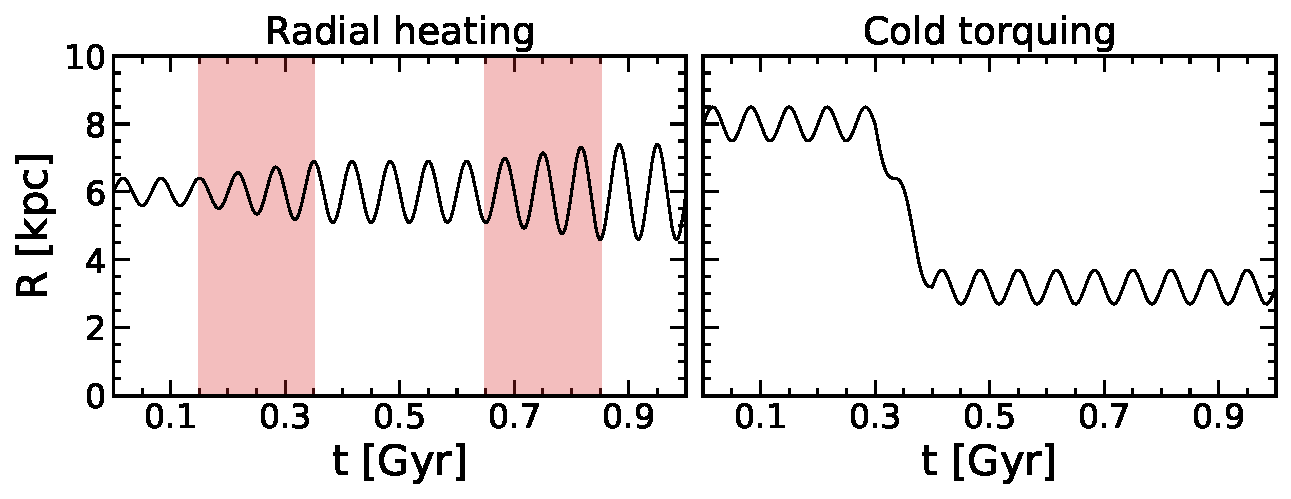
\includegraphics[width=1\textwidth]{images/radialmigration.pdf}
    \caption{A simple sketch of the radius evolution of an orbit that undergoes radial migration. \textit{Left}: Shows the effect of radial heating or blurring, which increases or decreases the amplitude of the radial oscillations of the orbit. The shaded regions mark the time during which the radial heating occurs. The guiding center radius, $R_g$, is never changed during the process. \textit{Right}: The effect of cold torquing or churning on an orbit, which displaces the guiding center radius, $R_g$, but does not increases the amplitude of oscillations and therefore does not increase the radial action, $J_R$.} % Fig. 1.4
    \label{fig:radialmigration}
\end{figure}

One rather simple cause of radial migration is what is called \textit{radial heating}, sometimes called \textit{blurring}. Stars are born in Giant Molecular Clouds (GMCs) which move on nearly circular orbits around the disk. This means that the stars themselves are born on nearly circular orbits. But through the evolution of stellar orbits they can scatter by interaction with things like other GMCs or clusters which will lead them onto eccentric orbits, called \textit{epicycle orbits} as they are described by the \textit{epicycle approximation}. The epicycle refers to the radial oscillations of the perturbed orbit, occuring with an \textit{epicycle frequency}, $\kappa$. The reason a perturbed star does not simply move to a different radius when scattered is because of the fine balance between centrifugal and gravitational force keeping it in place. If the star is pushed radially outwards, the centrifugal force decreases faster than gravity and the star moves back in. The star now overshoots to an interior radius where the centrifugal force increase faster than gravity which pushes it back out. In other words we say that the star is stable to small velocity changes. Because of the oscillations the star will visit different radii than its original radius, called the \textit{guiding radius}, $R_g = L_z / v_c$, where $L_z$ is the angular momentum perpendicular to the disk and $v_c$ is the circular velocity. It is the process of increasing the amplitude of the oscillations that we call radial heating and we show how this might look in the left panel of \ref{fig:radialmigration}. 

Given that the stars visit other regions of the Galaxy, they can obviously enrich those regions as well which leads to the conclusion that radial heating can contribute to the width observed in the chemical evolutionary tracks discussed in the previous section. It can be shown as in \cite{binney:07} however that radial heating will only account for around 50\% of the observed scatter in the metallicity and instead there must be some additional source of mixing to explain the measured scatter. 

\subsection{Cold torquing}
\begin{figure}[t]
    \centering
    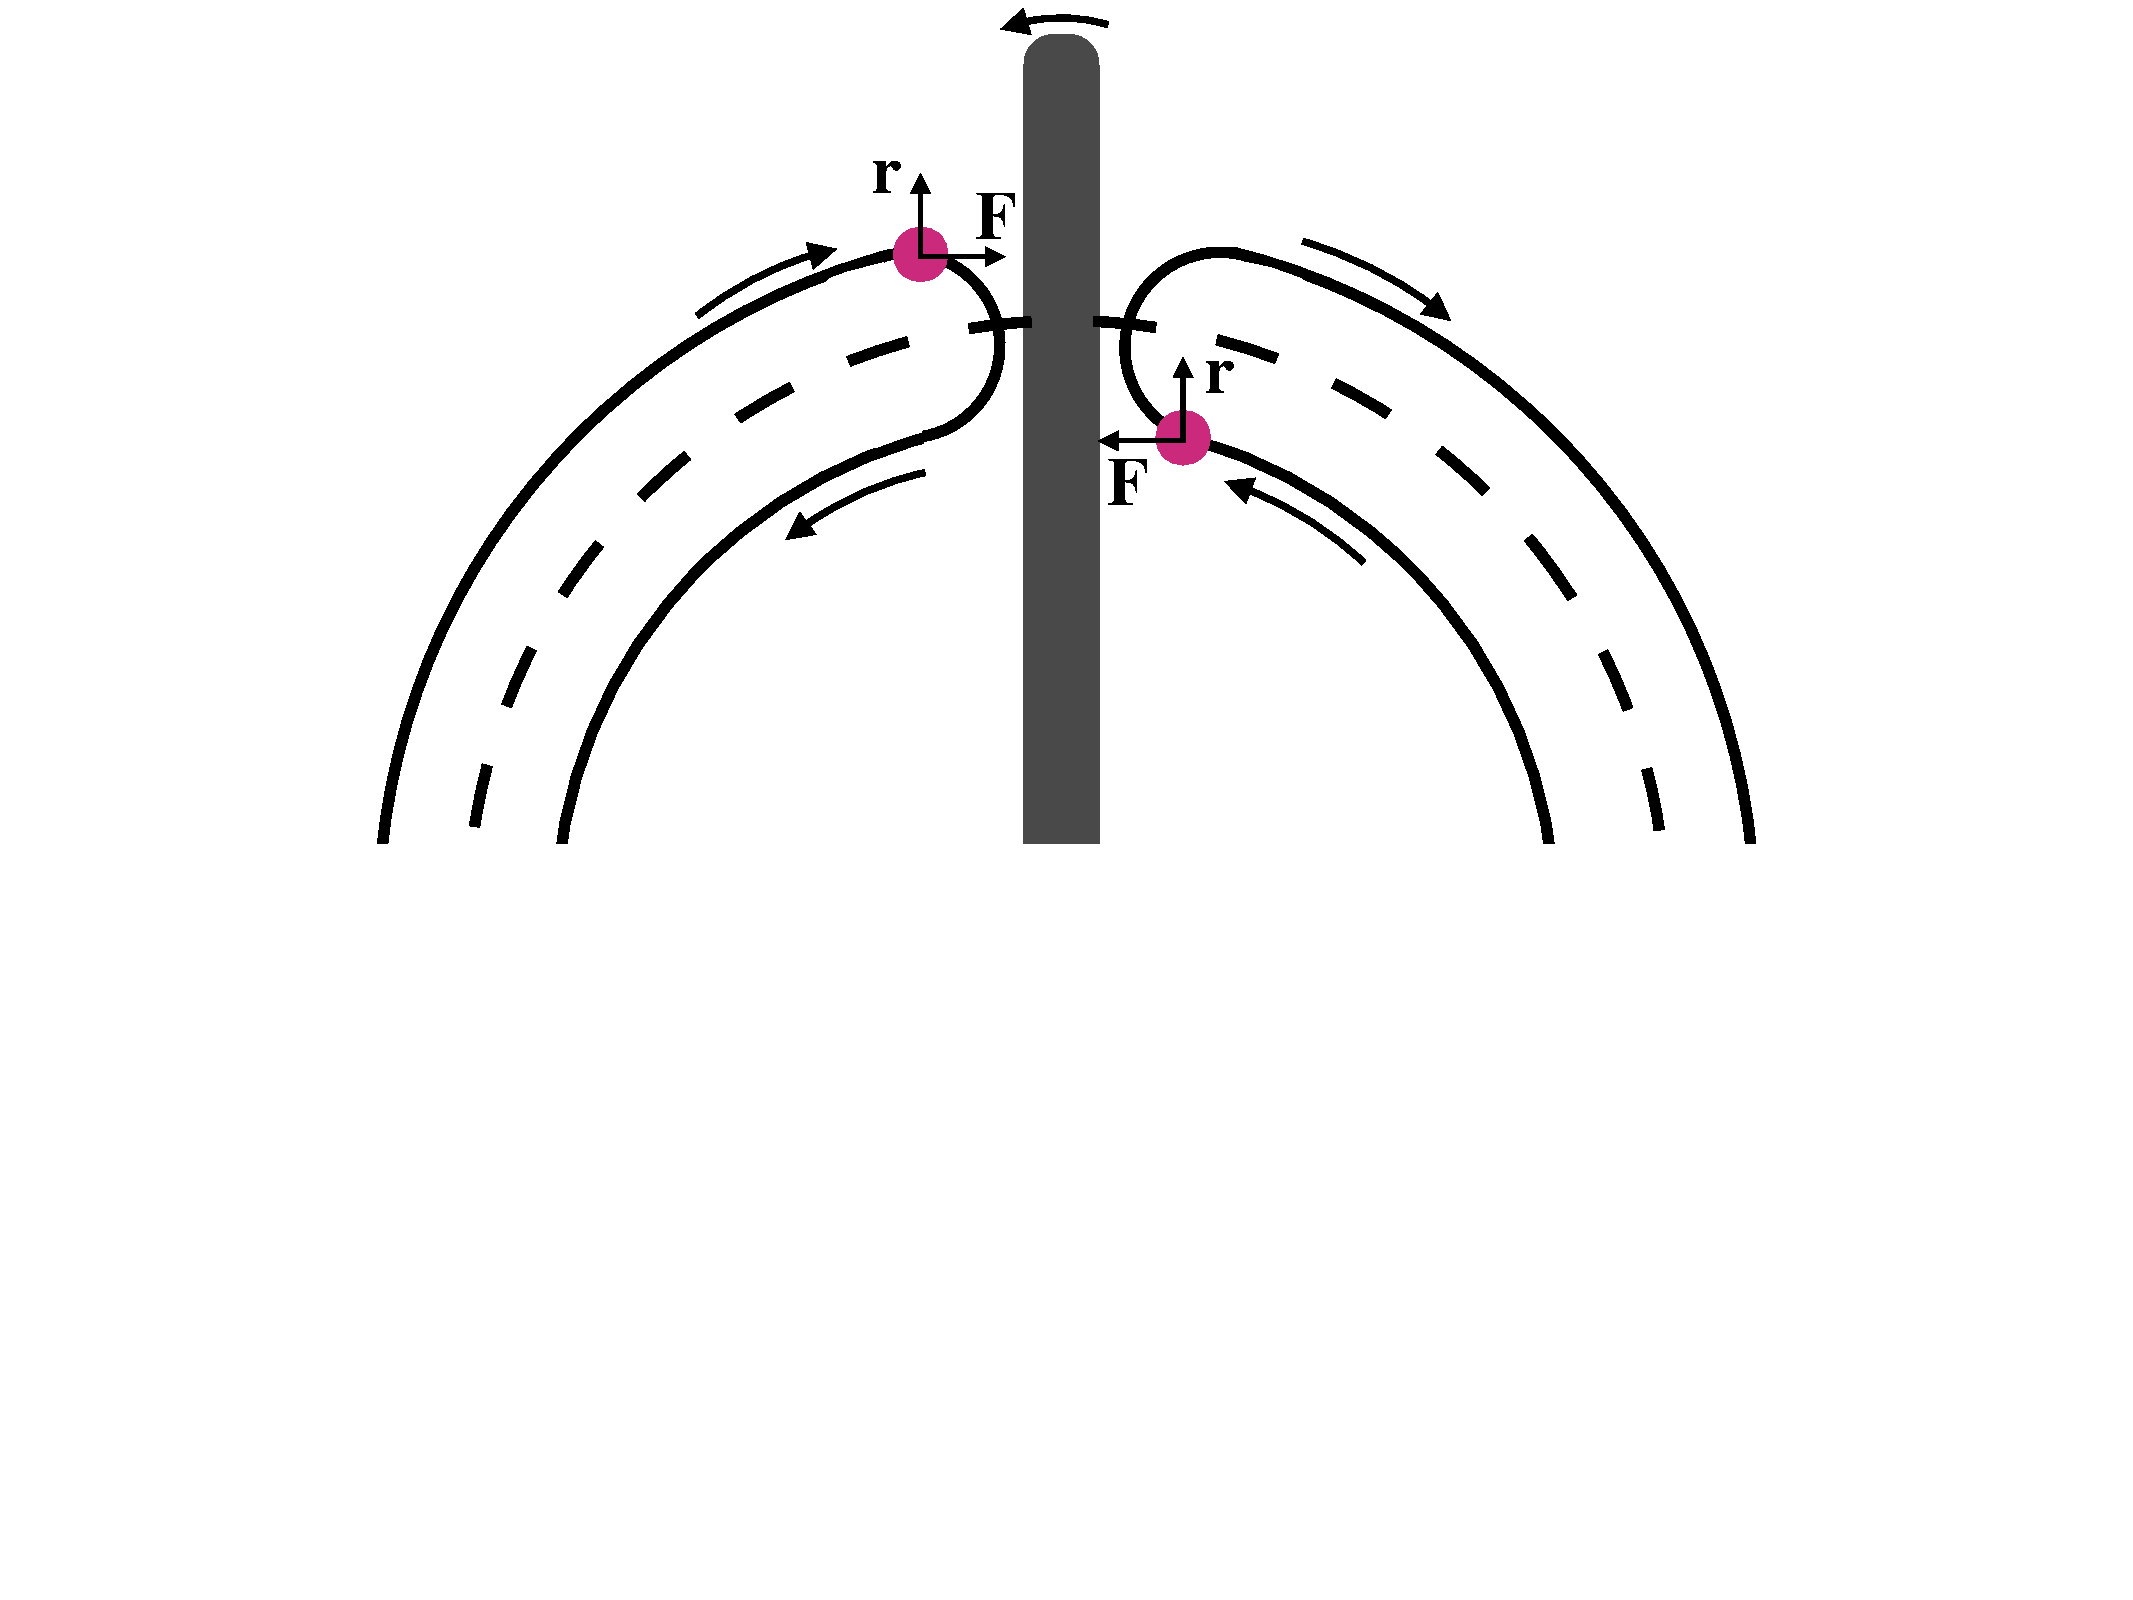
\includegraphics[width=0.8\textwidth]{images/torquing.pdf}
    \caption{The concept of horseshoe orbits and angular momentum transfer near corotation of a non-axisymmetric feature with constant angular speed. The dashed line marks the corotation radius and the pink points are positions along the horseshoe orbit right before angular momentum transfer. The vectors for $\pmb{r}$ and $\pmb{F}$ which gives the torque is indicated} % Fig. 1.5
    \label{fig:torquing}
\end{figure}
Another source of radial mixing was described first in a seminal paper by \cite{sellwood:02} wherein it was shown that disk heating is not the dominant effect of the spiral arms. Instead, non-axisymmetric features like the bar and spiral arms are able to shift the guiding radii of stars without significantly altering their dynamics. This processes occurs through resonant interactions with the non-axisymmetric features. The spiral arms or bar will exert a torque that changes the angular momentum of the star's orbit since:
\begin{equation}
    \frac{d}{dt}\pmb{L} = \frac{d}{dt}(\pmb{r}\times\pmb{p}) = \pmb{r}\times\pmb{F} = \pmb{\Gamma}.
\end{equation}
Axisymmetric features like bars and spirals move with constant angular velocity, which means that the non-angular velocity increases further out. This means that for stars with approximately constant circular velocity there is a radius at which the velocity of a star and spiral/bar is the same, called \textit{corotation}. Beyond this point stars move more slowly than the spiral and within it they move faster. Faster stars catch up to the feature and will have a force, $\pmb{F}$, directed towards it. Slower stars instead fall into it with a force in the opposite direction. We illustrate this in Fig. \ref{fig:torquing} which shows that for the fast stars, the torque will be directed inwards, i.e., negative which decreases the angular momentum and transfers it to a smaller $R_g$ orbit where it moves faster. It eventually catches up to the spiral/bar and is given a positive torque, migrating outwards. In this simple view the orbit would go back and forth but due to the transient nature of spiral arms and the plurality of axisymmetric features, this is not a likely outcome.

\begin{figure}[t]
    \centering
    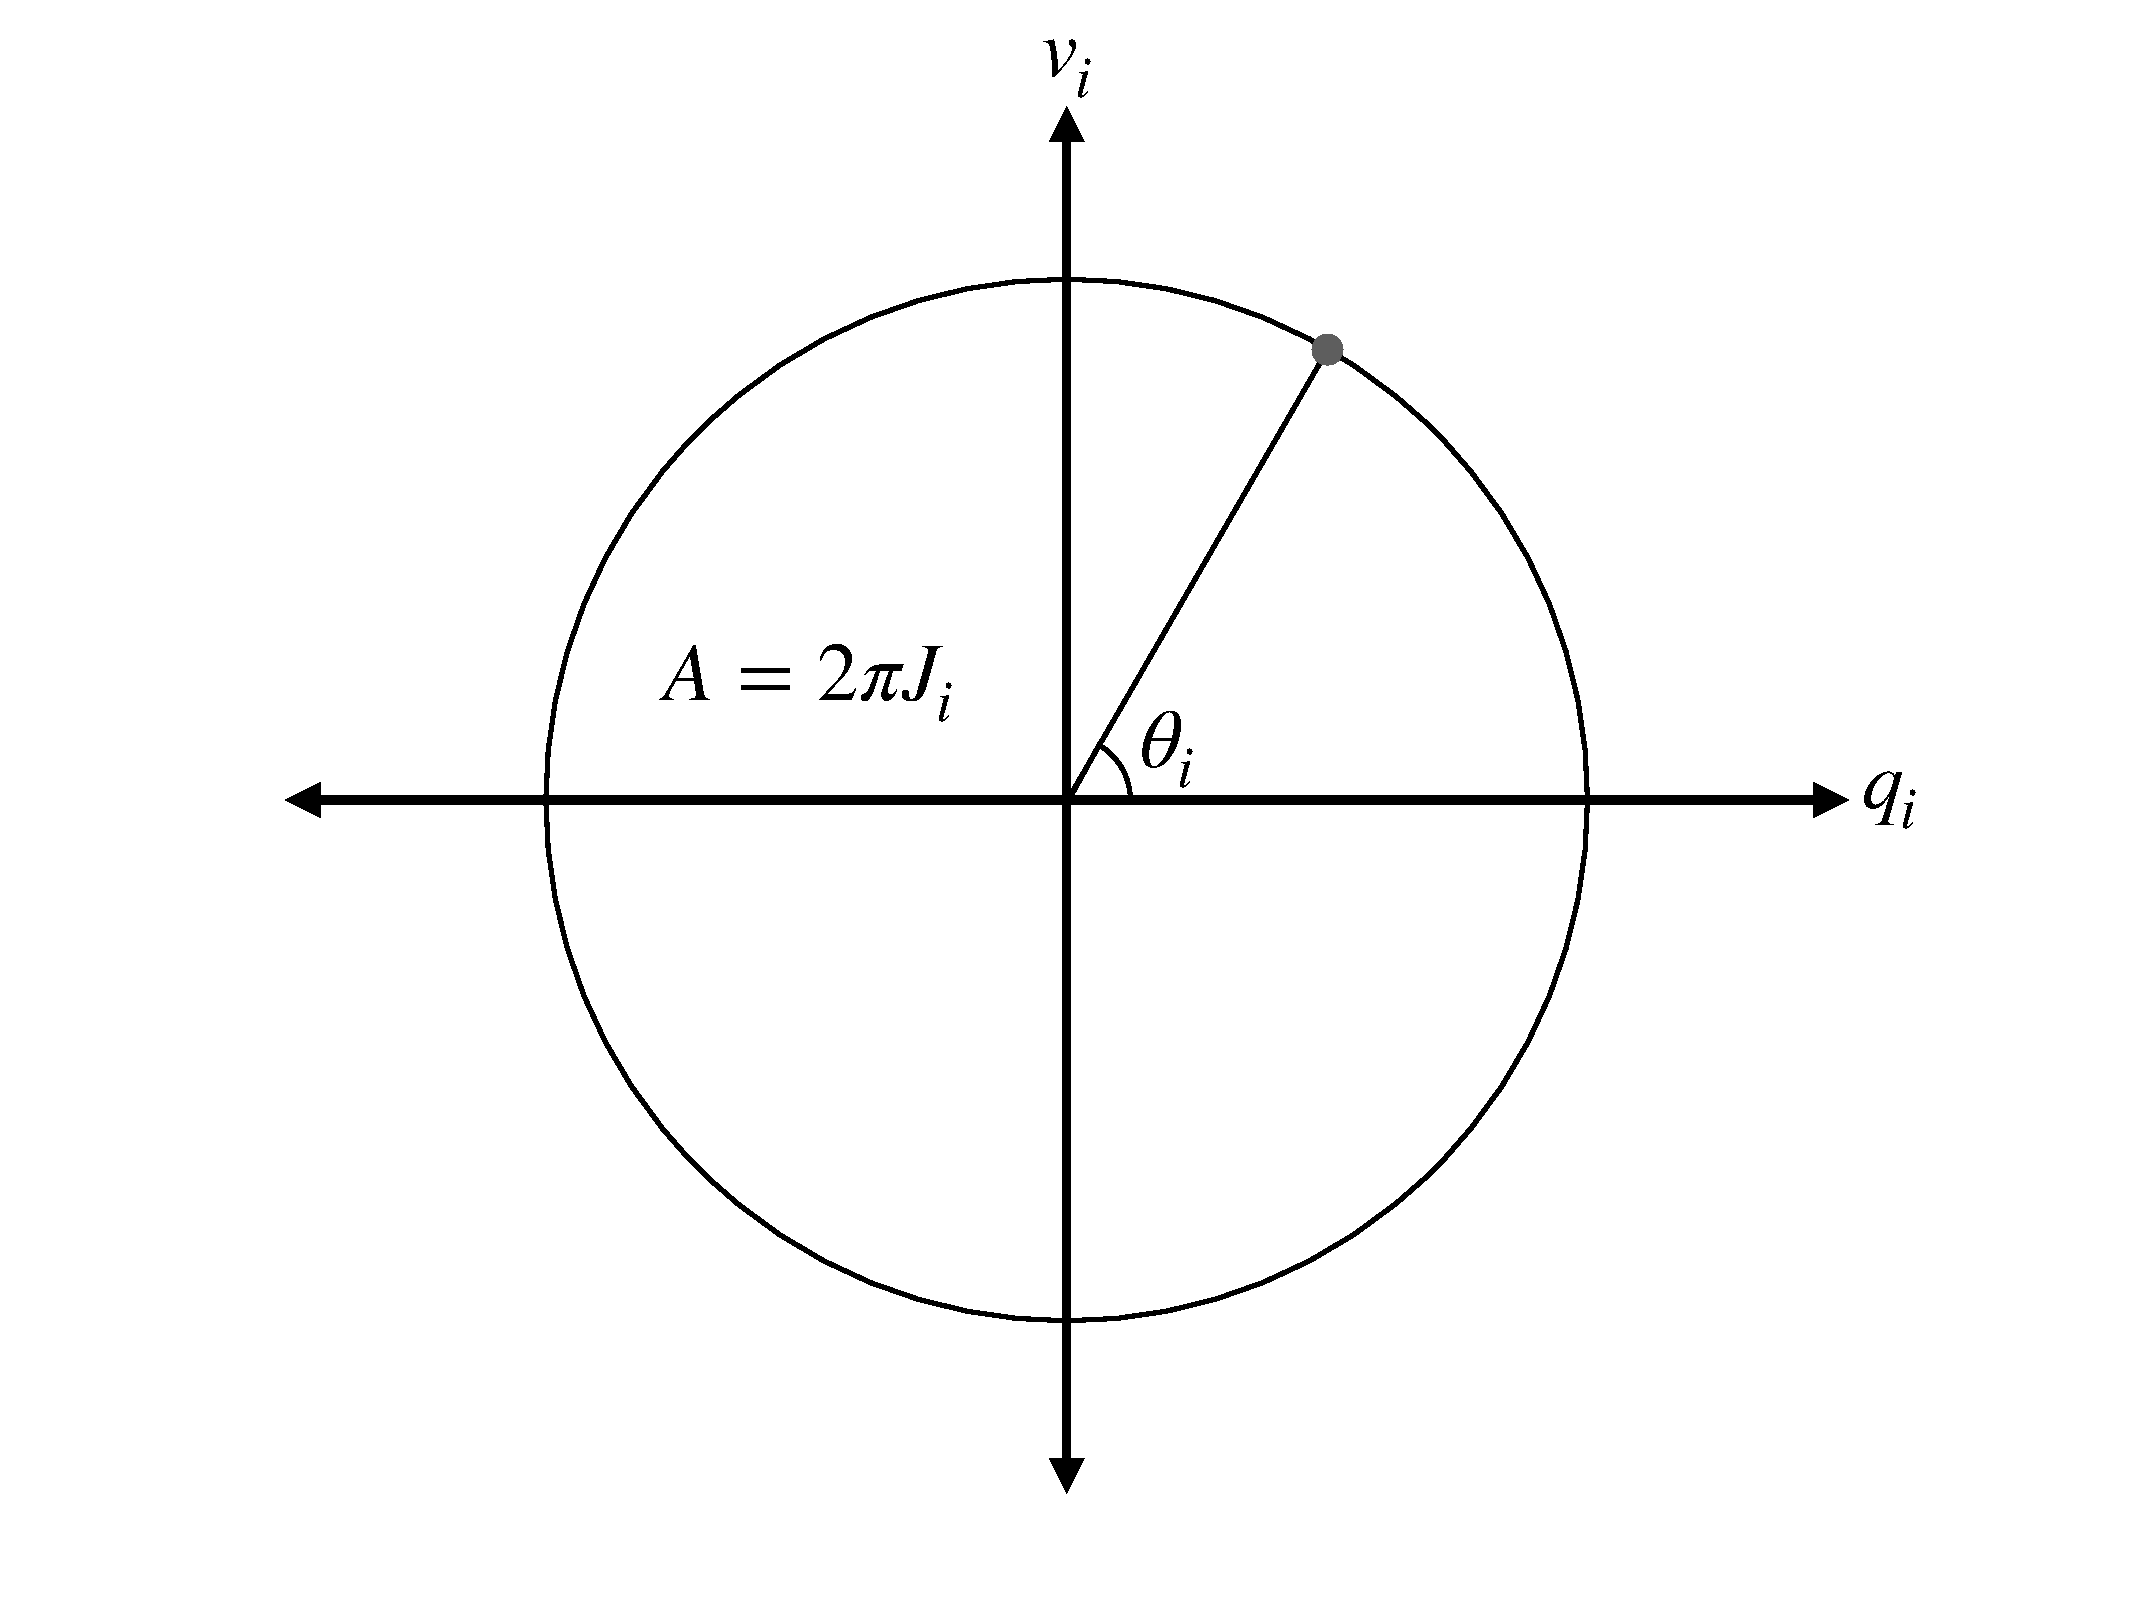
\includegraphics[width=0.6\textwidth]{images/actionangle.pdf}
    \caption{A polar coordinate analogy of action-angle variables to phase-space coordinate. An orbit oscillating in some coordinate $q_i$ will have a velocity, $v_i$ which also oscillates. A point on the same orbit can be described with a constant area, $2\pi J_i$ and an angle $\theta_i$.} % Fig. 1.6
    \label{fig:actionangle}
\end{figure}

This provides the `torquing' part. The cold part of the term comes from the fact that the migration does not increase the random motion of the affected stars, leaving them kinematically unscathed from the interaction. To properly explain this concept, we introduce \textit{action-angle} variables to describe a stellar orbit. A simple polar-coordinate analogy is given in Fig. \ref{fig:actionangle} which shows that an orbit in a certain dimension, $i$, can be described with two oscillating phase-space coordiantes $(q_i, v_i)$ or one constant and one oscillating, $(J_i, \theta_i)$.

If we place ourselves in the rotating frame of a Galaxy, moving with a pattern speed $\Omega_p$ relative to the intertial frame, we can describe its total energy or Hamiltonian, $E_J$, using the Hamiltonian of the inertial frame, $E$:
\begin{equation}\label{eq:jacobi}
    E_J = E - \Omega_pL,
\end{equation}
Where $L$ is the angular momentum. We call $E_J$ the \textit{Jacobi integral} (see \citealt{binney:08} chapter 3.3.2 for a full derivation) and it is constant in time. So the different between two moments is:
\begin{equation}
    \Delta E = \Omega_p\Delta L,
\end{equation}
which itself can be split into radial and azimuthal energy parts
\begin{equation}\label{eq:Echange}
    \Delta E = \frac{\partial H}{\partial L}\Delta L + \frac{\partial H}{\partial J_R}\Delta J_R,
\end{equation}
where $J_R$ is the \textit{radial action}. If we use Hamilton's equations with $\pmb{J}$ as the momentum and $\pmb{\theta}$ as the coordinate we find:
\begin{equation}
    \dot{J}_i = - \frac{\partial H}{\partial \theta_i} = 0 \qquad \dot{\theta}_i = \frac{\partial H}{\partial J_i} = \Omega_i,
\end{equation}
where $\Omega_i$ is an angular velocity. We have that $\partial H / \partial J_r = \omega_R$ and $\partial H / \partial L = \Omega$, the radial and azimuthal frequencies. Combining this with eq. \eqref{eq:Echange} gives
\begin{equation}
    \Delta E = \Omega\Delta L + \omega_R \Delta J_r,
\end{equation}
which when put into eq. \eqref{eq:jacobi} yields
\begin{equation}\label{eq:churning}
    \Delta J_r = \frac{\Omega_p - \Omega}{\omega_R}\Delta L.
\end{equation}
It is the implications of eq. \eqref{eq:churning} that provides the `cold' part. Stars have almost constant circular velocity across the disk which means that angular momentum corresponds to guiding radius, $L_z \propto R_g$. We know that torquing provides a change in the angular momentum from our discussion above, so this will correspond to a change in the radial action of the orbit, unless the angular velocity of the star matches that of the axisymmetric feature, $\Omega = \Omega_p$, which is the case near corotation. This behaviour was demonstrated and detailed in \cite{sellwood:02} which showed also that the migration caused by the cold torquing can displace the star on kiloparsec scales, without imparting any increased motions. The nature of cold torquing is therefore not only impressive but also frustrating since if stars are able to change their guiding radius by such scales without having any kinematic evidence of such a process, the history of different regions of the Galaxy become much more complex. 

It is worth mentioning the other resonances that exist besides corotation. A particularly strong such resonance is when the radial frequency, $\omega_R$ (identical to $\kappa$ in the epicyclic approximation), is a multiple of the frequency with which the star encounters the non-axisymmetric feature $(\Omega_p - \Omega)$. In other words when
\begin{equation}
\omega_R = \pm m(\Omega_p - \Omega).
\end{equation}
These resonances are called \textit{Lindblad resonances} after Swedish astronomer Bertil Lindblad (1895 - 1965). The positive sign corresponds to an orbit in which the rotating feature sweeps by the slower star as it completes $m$ radial oscillations and is known as an \textit{Outer Lindblad Resonances} (OLR). The negative sign is when the fast star rotates past the rotating feature by the time it completes its $m$ radial osscillations and is then called an \textit{Inner Lindblad Resonance} (ILR). At these resonances we have from eq. \eqref{eq:churning}
\begin{equation}
    \Delta J_r = \pm \frac{1}{m}\Delta L,
\end{equation}
which shows how migration at these resonances increases the radial action, therefore making them a potential source of migration by radial heating as discussed previously.

Clearly, must understand how stars are radially migrated. In particular, the process of cold torquing must be well understood since it is unique in the fact that it leaves no dynamical trace. Without these insights we cannot have a full picture of the history and evolution of our Galaxy.